\section{Laboratory work implementation}

\subsection{Tasks and Points}
\begin{itemize}
	\item Basic Level (nota 5 || 6):
	
	\begin{itemize}
		\item Realizeaza un mini site cu 3 pagini statice
	\end{itemize}
	
	\item Normal Level (nota 7 || 8):
	
	\begin{itemize}
		\item ISite-ul trebuie sa pastreze toata informatia intr-o baza de date
	\end{itemize}
	\item Advanced Level (nota 9 || 10):
	
	\begin{itemize}
		\item Site-ul trebuie sa contina AJAX Requests.
    	\item Implimentarea XHR sau JSON responses. Careva din informatie trebuie sa fie dinamic incarcata pe pagina.
	\end{itemize}
\end{itemize}
    



\subsection{Analiza lucrarii de laborator}

Linkul la repozitorul Github:\\
\begin{center}
\url{https://github.com/aillyroredshi/MIDPS}
\end{center}

Am utilizat un host online pentru a tine webapp-ul si fisierele sale necesare.
\begin{center}
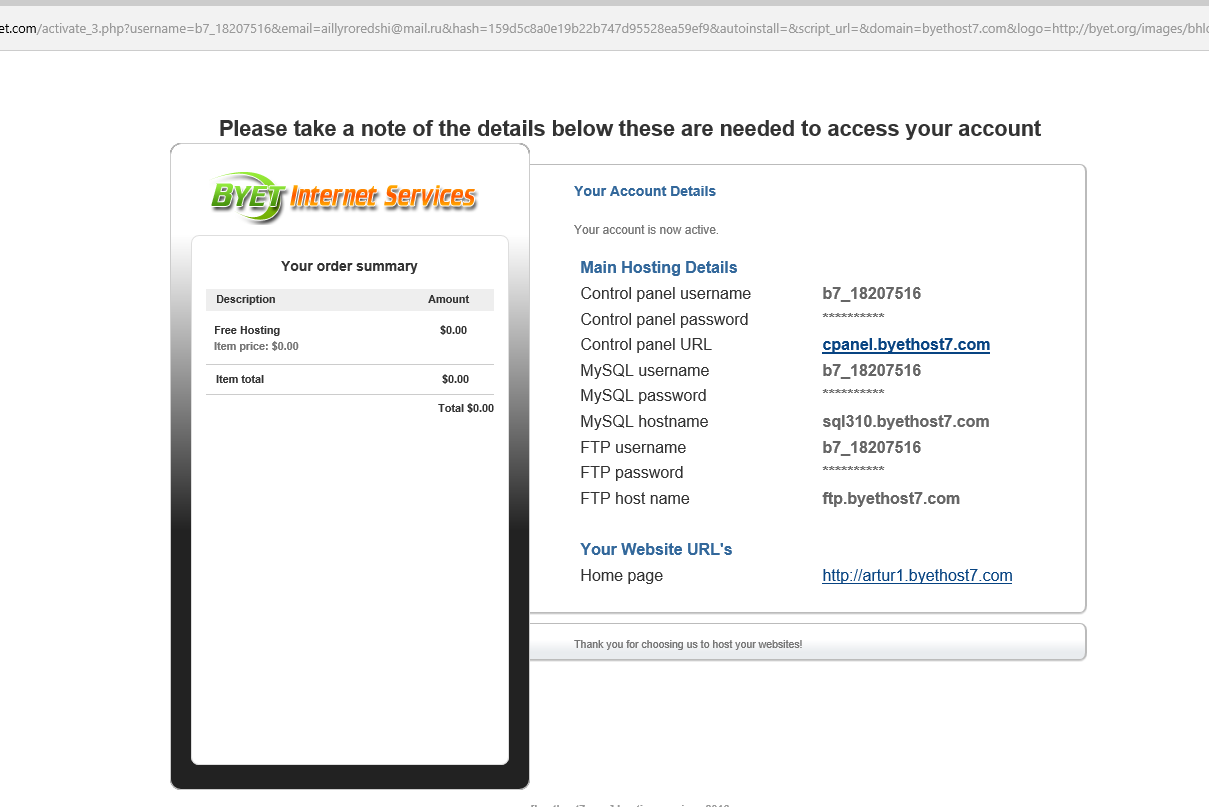
\includegraphics[scale=0.5]{images/123}
\end{center}
Pentru inceput am realizat trei fisiere html:pagina principala,portofoliu si mini\_store.Toate aceste pagini sunt interactive si isi schimba marimea dupa device-ul folosit datorita ca am utilizat foundation.zurb care la-m modificat dupa necesitatile mele.
\begin{flushleft}
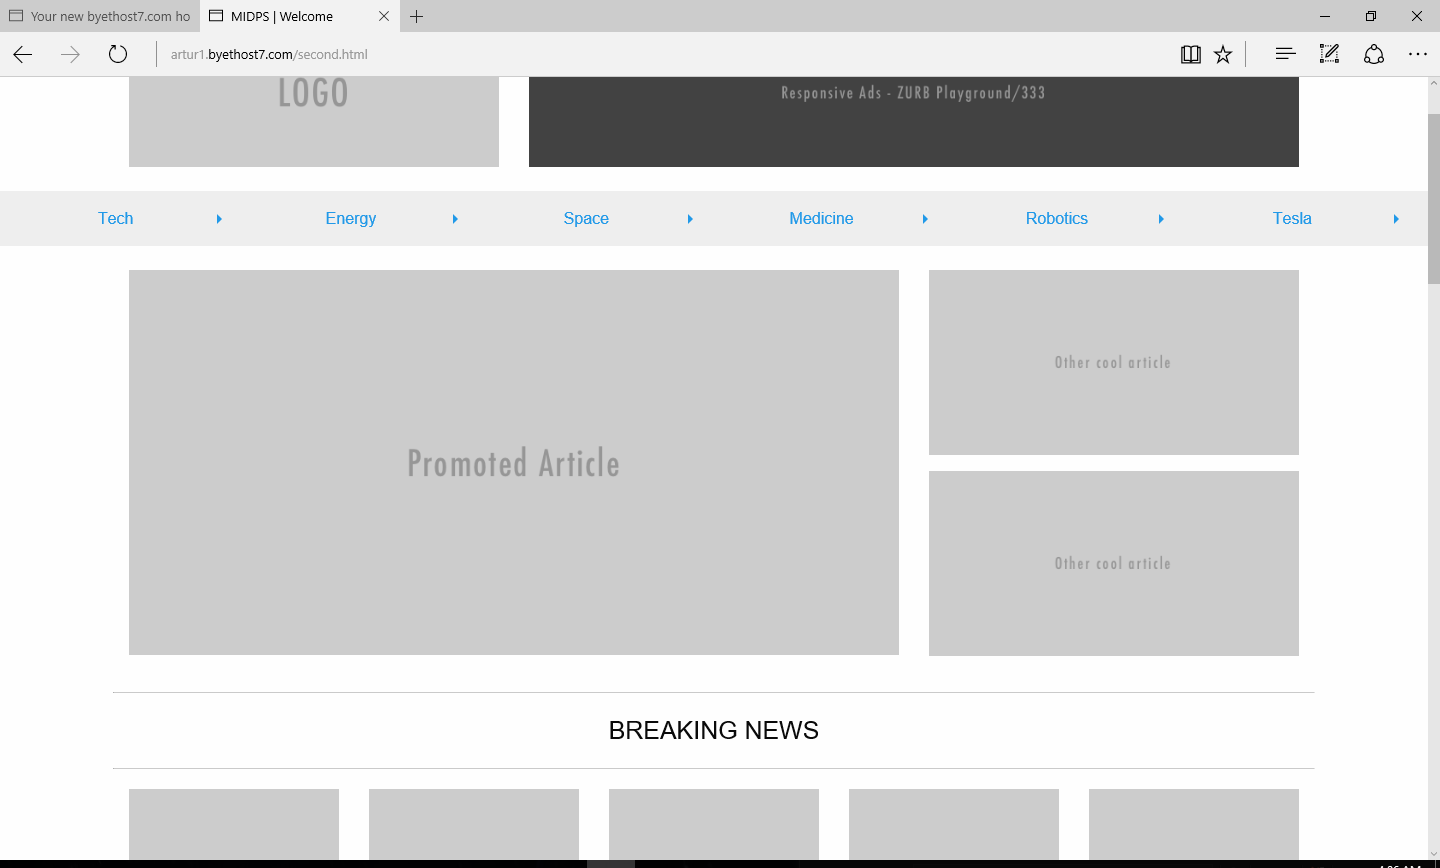
\includegraphics[scale=0.5]{images/1}
\end{flushleft}
\begin{flushleft}
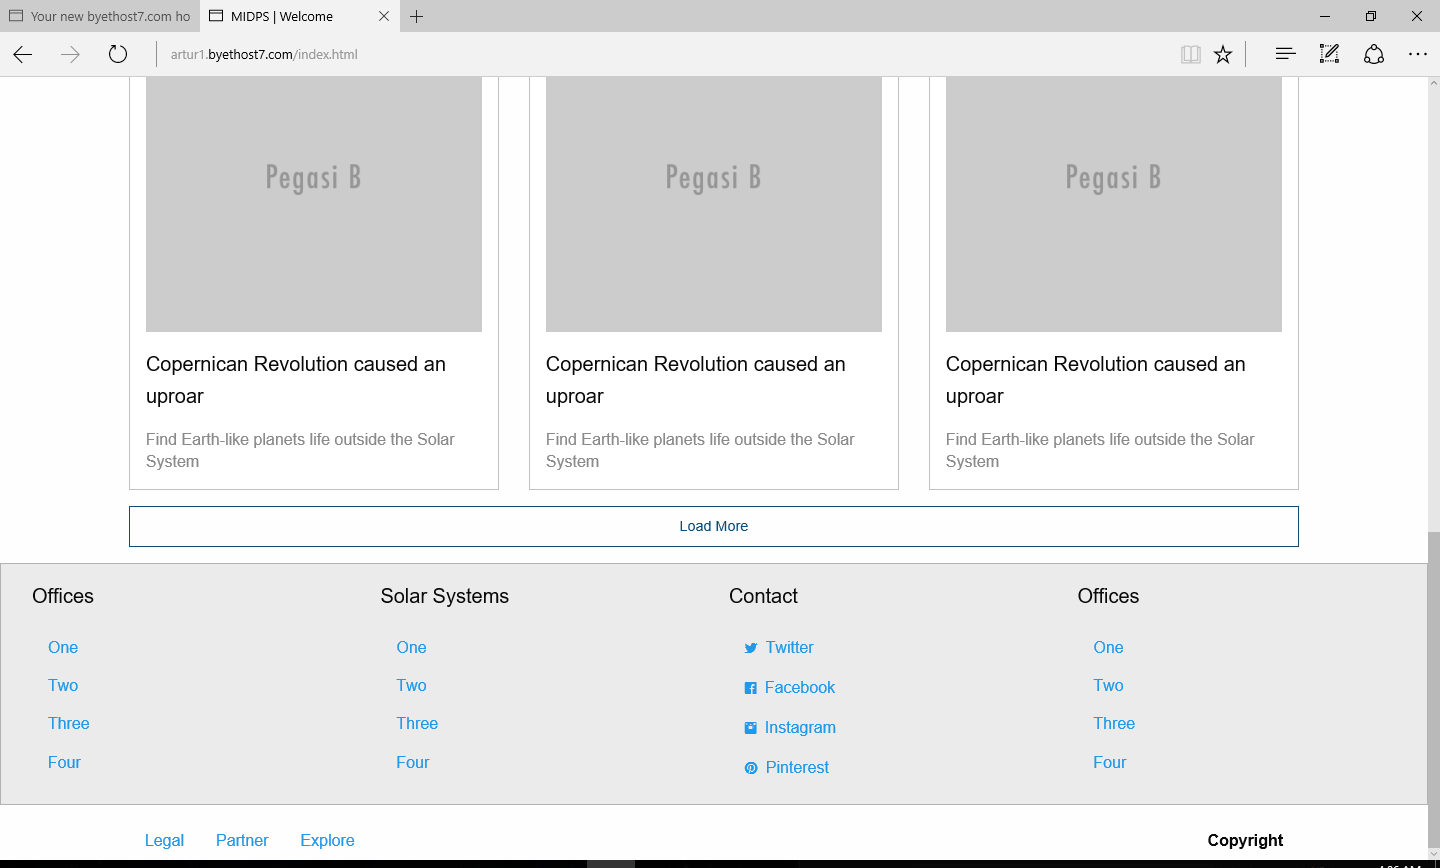
\includegraphics[scale=0.5]{images/2}
\end{flushleft}
\begin{flushleft}
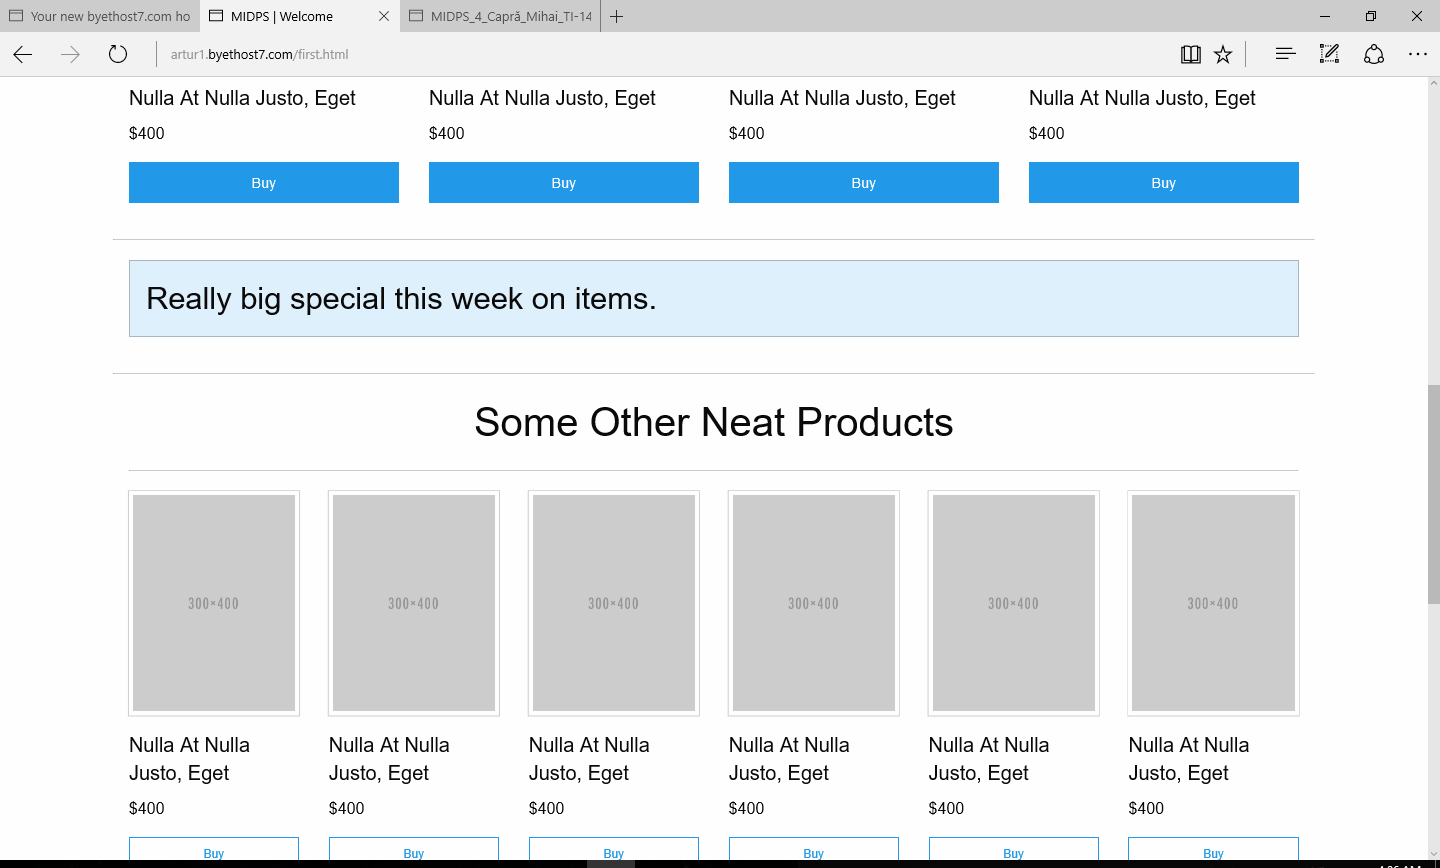
\includegraphics[scale=0.5]{images/3}
\end{flushleft}
Dupa aceasta am configurat o baza de date cu componentele necesare(username,password,db\_name)  

\begin{center}
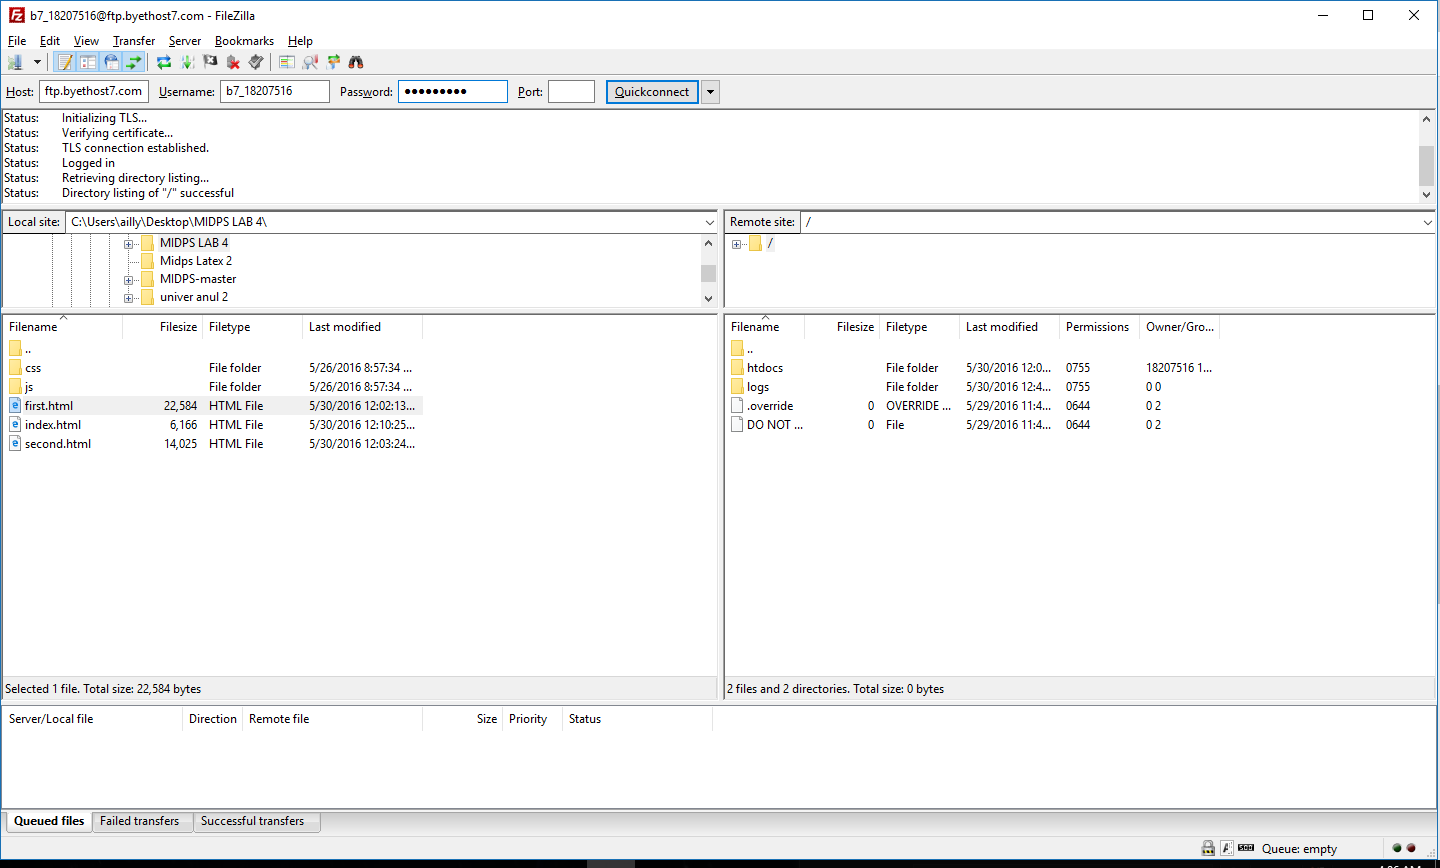
\includegraphics[scale=0.6]{images/4}
\end{center}
\clearpage